\documentclass[border=10pt]{standalone} 
\usepackage{verbatim}
\usepackage{tikz}
\tikzset{
  treenode/.style = {shape=rectangle, rounded corners,
                     draw, align=center,
                     top color=white, bottom color=blue!20},
  root/.style     = {treenode, font=\Large, bottom color=red!30},
  env/.style      = {treenode, font=\ttfamily\normalsize},
  dummy/.style    = {circle,draw}
}
\begin{document}
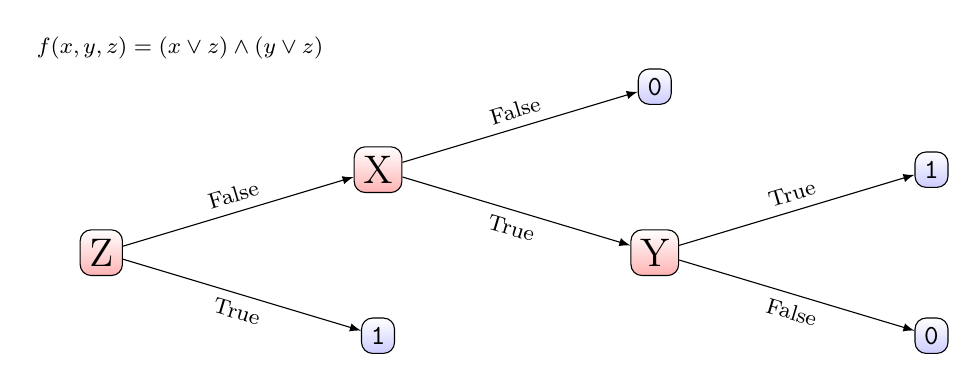
\begin{tikzpicture}
  [
    grow                    = right,
    sibling distance        = 6em,
    level distance          = 10em,
    edge from parent/.style = {draw, -latex},
    every node/.style       = {font=\footnotesize},
    sloped
  ]
  \node at (1,2.6) {$ f(x,y,z) = (x\lor z) \land (y\lor z)$};
  \node [root] {Z}
    child { node [env] {1}
      edge from parent node [below] {True} }
    child { node [root] {X}
      child { node [root] {Y}
        child { node [env] {0}
          edge from parent node [below] {False} }
        child { node [env] {1}
                edge from parent node [above] {True} }
        edge from parent node [below] {True} }
      child { node [env] {0}
              edge from parent node [above, align=center]
                {False}
              node [below] {}}
              edge from parent node [above] {False} };
\end{tikzpicture}
\end{document}